\documentclass[11pt,compress,t,notes=noshow, aspectratio=169, xcolor=table]{beamer}

\usepackage{../../style/lmu-lecture}
% Defines macros and environments
% This file is included in slides and exercises

% Rarely used fontstyle for R packages, used only in 
% - forests/slides-forests-benchmark.tex
% - exercises/single-exercises/methods_l_1.Rnw
% - slides/cart/attic/slides_extra_trees.Rnw
\newcommand{\pkg}[1]{{\fontseries{b}\selectfont #1}}

% Spacing helpers, used often (mostly in exercises for \dlz)
\newcommand{\lz}{\vspace{0.5cm}} % vertical space (used often in slides)
\newcommand{\dlz}{\vspace{1cm}}  % double vertical space (used often in exercises, never in slides)
\newcommand{\oneliner}[1] % Oneliner for important statements, used e.g. in iml, algods
{\begin{block}{}\begin{center}\begin{Large}#1\end{Large}\end{center}\end{block}}

% Don't know if this is used or needed, remove?
% textcolor that works in mathmode
% https://tex.stackexchange.com/a/261480
% Used e.g. in forests/slides-forests-bagging.tex
% [...] \textcolor{blue}{\tfrac{1}{M}\sum^M_{m} [...]
% \makeatletter
% \renewcommand*{\@textcolor}[3]{%
%   \protect\leavevmode
%   \begingroup
%     \color#1{#2}#3%
%   \endgroup
% }
% \makeatother


\title{Interpretable Machine Learning}
% \author{LMU}
%\institute{\href{https://compstat-lmu.github.io/lecture_iml/}{compstat-lmu.github.io/lecture\_iml}}
\date{}

\begin{document}

\newcommand{\titlefigure}{figure/gam_effects.pdf}
\newcommand{\learninggoals}{
\item Generalized additive model
% \item Decision trees
% \item Other interpretable models}
\item Model-based boosting with simple base learners
\item Feature effect and importance in model-based boosting}

\lecturechapter{GAM \& Boosting}
\lecture{Interpretable Machine Learning}

%------------------------------------------------------------------
%------------------------------------------------------------------

\begin{frame}{Generalized Additive Model (GAM) \citebutton{Hastie and Tibshirani (1986)}{https://www.jstor.org/stable/2245459}}

\textbf{Problem}: LM not great if features act on outcome non-linearly % $\leadsto$ standard 

\begin{columns}[totalwidth=\textwidth]
    \begin{column}{0.55\textwidth}
    
        \only<2->{
        \textbf{Workaround in LMs / GLMs}: 
        \begin{itemize}
            \item Feature transformations (e.g., exp or log)
            \item Including high-order effects
            \item Categorization of features (i.e., intervals/ buckets of feature values)
        \end{itemize}}
    \end{column}
    \begin{column}{0.45\textwidth}
        \begin{center}
            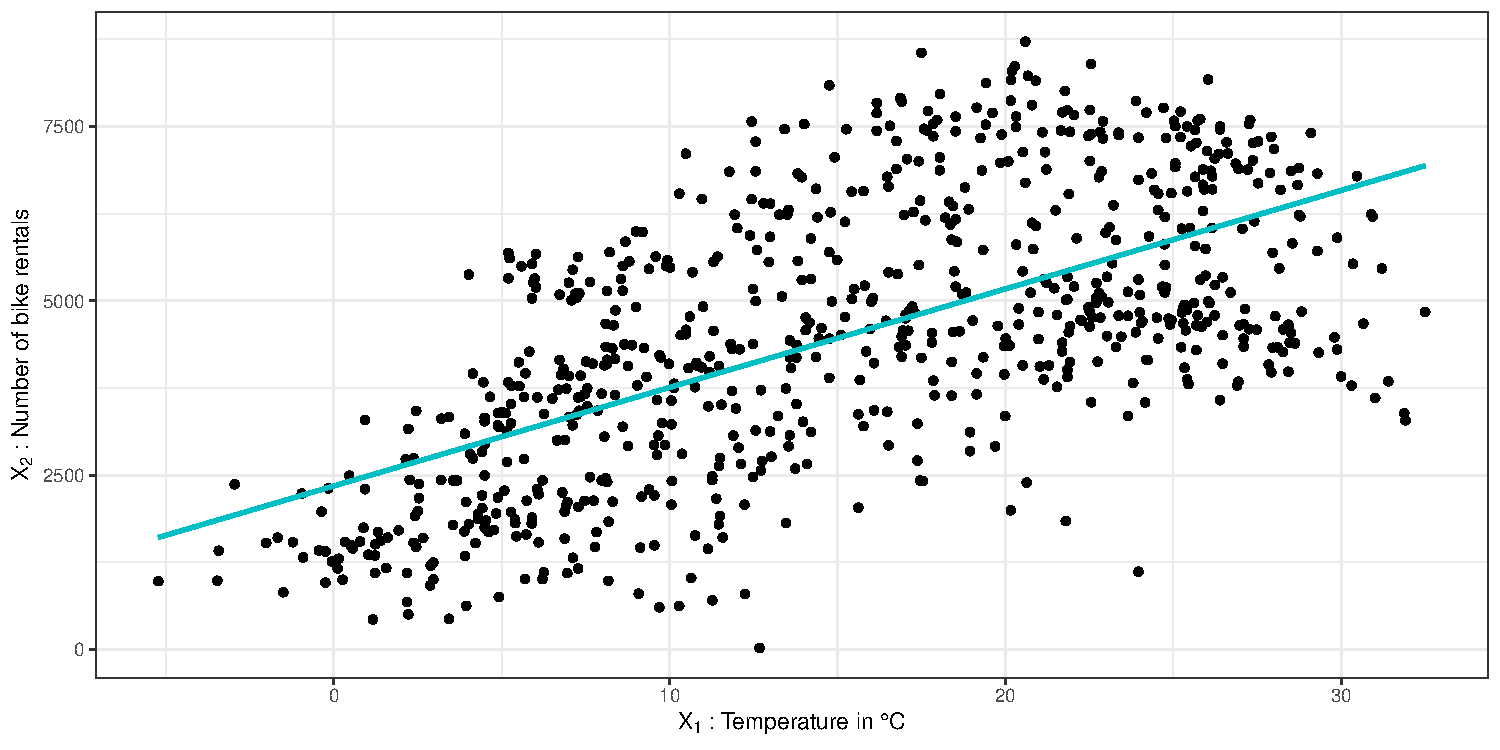
\includegraphics[width = .95\textwidth]{figure/intro_lm_bike.pdf}
            %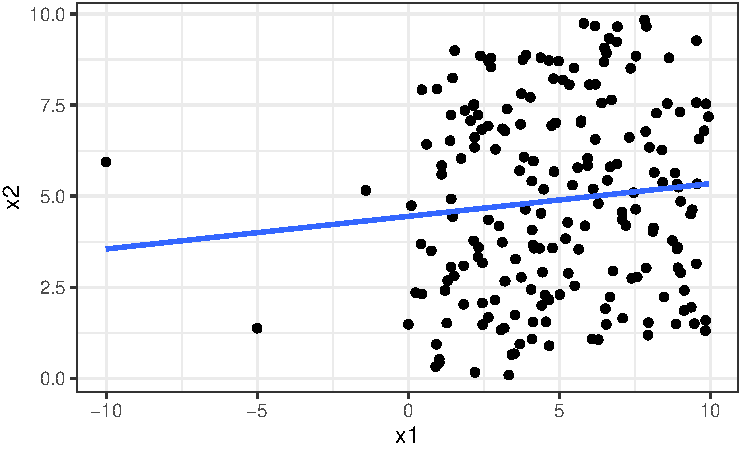
\includegraphics[width = \textwidth]{figure/lm_bad_fit2.pdf}
        \end{center}
    \end{column}
\end{columns}

%\medskip

\only<3->{
\textbf{Idea of GAMs:}

    \begin{itemize}
        \item Instead of linear terms $\theta_j x_j$, use flexible functions $f_j(x_j)$ $\leadsto$ splines
            $$g(\E (y \mid \xv)) = \theta_0 + f_1(x_1) + f_2(x_2) + \ldots + f_p(x_p)$$
    
        \item Preserves additive structure and allows to model non-linear effects
        \item Splines have a smoothness parameter to control flexibility (prevent overfitting)\\
        $\leadsto$ Needs to be chosen, e.g., via cross-validation
    \end{itemize}}   

\end{frame}


\begin{frame}{Generalized Additive Model (GAM) - Example}
Fit a GAM with smooth splines for four numeric features of bike rental data \\
$\leadsto$ more flexible and better model fit but less interpretable than LM

\begin{columns}[T, totalwidth=\textwidth]
\begin{column}{0.5\textwidth}
\begin{table}[ht]
\centering
\scriptsize
% \begin{tabular}{rrrrr}
%   \hline
%  & edf & Ref.df & F & p-value \\ 
%   \hline
% s(temp) & 5.8 & 7.0 & 57.2 & 0.00 \\ 
%   s(hum) & 4.0 & 5.1 & 68.0 & 0.00 \\ 
%   s(windspeed) & 1.7 & 2.1 & 50.1 & 0.00 \\ 
%   s(days\_since\_2011) & 8.3 & 8.8 & 154.4 & 0.00 \\ 
%   \hline
\begin{tabular}{rrr}
  \hline
 & edf & p-value \\ 
  \hline
s(temp) & 5.8 & 0.00 \\ 
  s(hum) & 4.0 & 0.00 \\ 
  s(windspeed) & 1.7 & 0.00 \\ 
  s(days\_since\_2011) & 8.3 & 0.00 \\ 
   \hline
\end{tabular}
\end{table}


\textbf{Interpretation}
\begin{itemize}
    %\item If the temperature increases by 1 degree Celsius then the log odds of high number of bike rentals increase linearly by 0.3 c.p.
    \item Interpretation is performed visually and relative to average prediction
    %, also see PDPs
    \item Edf: effective degrees of freedom\\
    $\leadsto$ represents degree of smoothness/complexity
\end{itemize}
\end{column}
\hfill
\centering
\begin{column}{0.5\textwidth}
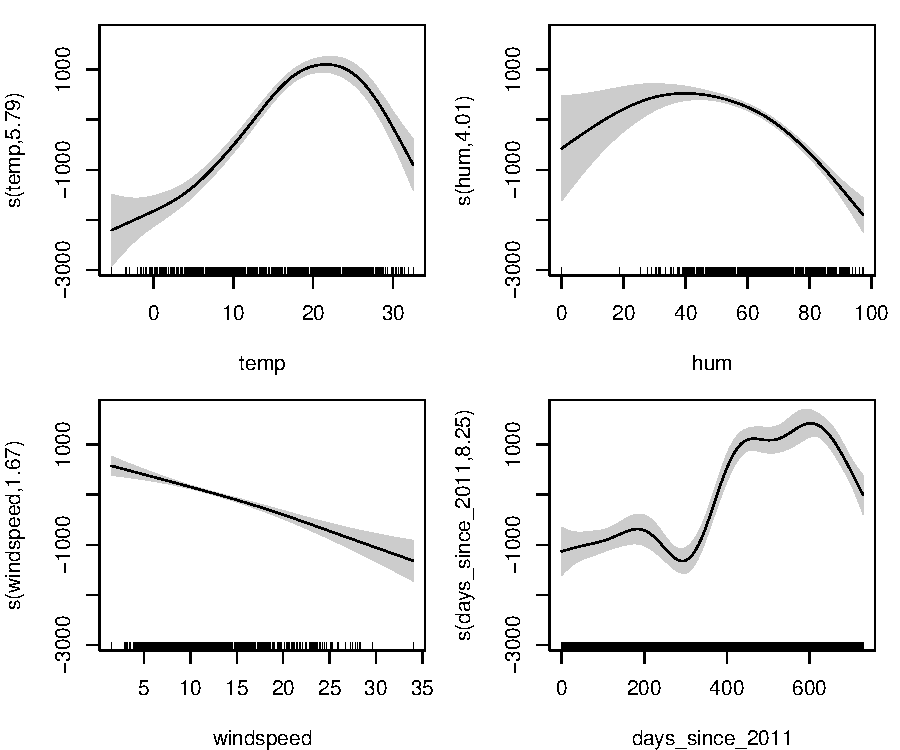
\includegraphics[width = \textwidth]{figure/gam_effects.pdf}
\end{column}
\end{columns}
\end{frame}

%------------------------------------------------------------------
%------------------------------------------------------------------

\begin{frame}{Model-based Boosting \citebutton{Bühlmann, Yu 2003}{https://doi.org/10.1198/016214503000125} \citebutton{Bühlmann, Hothorn 2008}{https://arxiv.org/abs/0804.2752}}

\begin{itemize}%[<+->]
%\setlength\itemsep{2em}
\item Boosting iteratively combines weak base learners to create powerful ensemble 
\item
Idea: Use simple BLs (e.g univariate, with splines) to ensure interpretability
%$\leadsto$ e.g., linear BL with single features in each iteration
%Boosting with gradient descent using interpretable base learners (e.g., use base learners with single features in each iteration $\leadsto$ coordinate gradient descent)
%The resulting ensemble is also interpretable.
%\pause
\item
Possible to combine BL of same type (with distinct parameters $\thetav$ and $\ts$):
%Two linear base learners $b_j(x, \theta)$ and $b_j(x, \theta^{\star})$ of the same type, but distinct parameter vectors $\theta$ and $\theta^{\star}$ can be combined in a base learner of the same type:
$$\bljt + \bljts = \bl[j](\xv, \thetav + \ts) $$
\pause
\item %In each iteration, a set of BLs is fitted on pseudo residuals. The one with the best fit is added to the previously computed model (using step-size $\nu$), e.g.,
In each iteration, fit a set of BLs, add best one to model (with step-size $\nu$):
%\medskip
\begin{align*}
\fmh[1] &= \hat{f}_0 + \nu \textcolor{blue}{\bl[3](\xv_3, \thetam[1])} \\
\fmh[2] &= \fmh[1] + \nu \textcolor{blue}{\bl[3](\xv_3, \thetam[2])} \\
%= \hat{f}_0 + \nu \textcolor{blue}{b_3(x_3, \theta^{[1]})} + \nu \textcolor{blue}{b_3(x_3, \theta^{[2]})}
\fmh[3] &= \fmh[2] + \nu \textcolor{orange}{\bl[1](\xv_1, \thetam[3])} \\
%= \hat{f}_0 + \nu \textcolor{blue}{b_3(x_3, \theta^{[1]})} + \nu \textcolor{blue}{b_3(x_3, \theta^{[2]})} + \nu \textcolor{orange}{b_1(x_1, \theta^{[3]})} 
&= \hat{f}_0 + \nu \left(\textcolor{blue}{\bl[3](\xv_3, \thetam[1] + \thetam[2])} + \textcolor{orange}{\bl[1](\xv_1, \thetam[3])}\right) 
\\
&= \hat{f}_0 + \textcolor{blue}{\hat{f}_3(\xv_3)} + \textcolor{orange}{\hat{f}_1(\xv_1)}
\end{align*}
\item Final model is additive GAM, we can read off effect curves
\end{itemize}
\end{frame}










\begin{frame}{Model-based Boosting - Linear Example}

Simple case: Use linear model with single feature (including intercept) as BL
$$
\bl[j](x_j, \thetav) = x_j\thetav + \thetav_0 \hspace*{0.2cm}\text{ for } j = 1,\ldots p \hspace*{0.3cm} \leadsto \text{ordinary linear regression}
$$

\begin{itemize}
\item<1-> Here: Interpretation of weights as in LM
\item<1-> After many iterations, it converges to same solution as LM %least square estimate of
\item<2-> Early stopping allows feature selection \& may prevent overfitting (regularization)
%\item Specifying loss and link function according to exponential family leads a (regularized) GLM
\end{itemize}
\begin{columns}[T, totalwidth=\textwidth]
\begin{column}{0.49\linewidth}
\scriptsize
\begin{table}[ht]
\centering
\tiny
\begin{tabular}{r|r|l}
  %\hline
\textbf{1000 iter. with $\nu = 0.1$} & Intercept & Weights \\ 
  \hline  \hline
days\_since\_2011 & -1791.06 & 4.9 \\ 
  \hline
  hum & 1953.05 & -31.1 \\ 
    \hline
  season & 0 &  \begin{tabular}[c]{@{}l@{}}
  WINTER: -323.4\\
  SPRING: 539.5\\
  SUMMER: -280.2\\
  FALL: 67.2
  \end{tabular}\\
    \hline
  %season &  & WINTER: -323.4, SPRING: 539.5, SUMMER: -280.2, FALL: 67.2 \\ 
  temp & -1839.85 & 120.4 \\ 
    \hline
  windspeed & 725.70 & -56.9 \\ 
    \hline
  offset & 4504.35 &  \\ 
   %\hline
\end{tabular}
\end{table}
% \centering
% $\Rightarrow$ Converges to solution of LM 
\end{column}
\begin{column}{0.49\linewidth}

\only<1>{\scriptsize
\medskip
Relative frequency of selected BLs across iterations
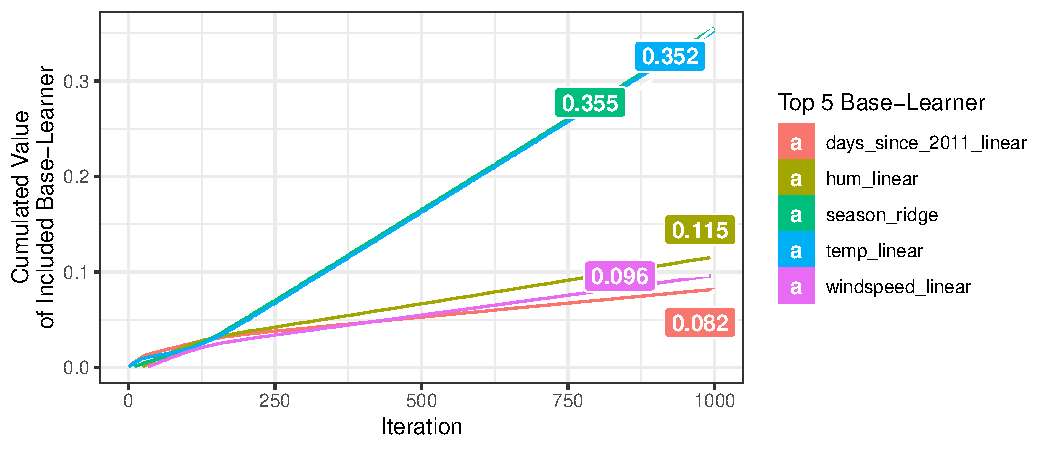
\includegraphics[width = .95 \linewidth]{figure/compboost_base_linear.pdf}}


\only<2>{
\begin{table}[ht]
\centering
\tiny
\begin{tabular}{r|r|l}
  %\hline
 \textbf{20 iter. with $\nu = 0.1$} & Intercept & Weights \\ 
  \hline  \hline
  days\_since\_2011 & -1210.27 & 3.3 \\ 
    \hline
   season & 0 & 
   \begin{tabular}[c]{@{}l@{}}
  WINTER: -276.9\\
  SPRING: 137.6\\
  SUMMER: 112.8\\
  FALL: 20.3
   \end{tabular}\\
     \hline
  temp & -1118.94 & 73.2 \\ 
    \hline
  offset & 4504.35 &  \\ 
   %\hline
\end{tabular}
\end{table}
% \centering
% \scriptsize
% $\Rightarrow$ 3 BLs selected after 20 iter. (feature selection)
}
\end{column}
\end{columns}

\begin{columns}[T, totalwidth=\textwidth]
\begin{column}{0.49\linewidth}
\scriptsize
\centering
$\Rightarrow$ Converges to solution of LM 
\end{column}
\begin{column}{0.49\linewidth}

\only<2>{
\centering
\scriptsize
$\Rightarrow$ 3 BLs selected after 20 iter. (feature selection)
}
\end{column}
\end{columns}
% \begin{itemize}
%     \item Linear base learners for numeric features and categorical base learner for season
%     \item 3 base learners selected after 100 iterations
% \end{itemize}

\end{frame}


\begin{frame}{Linear Example: Interpretation}

\medskip
\textbf{Feature importance:} aggregated change in risk in each iteration per feature
\begin{itemize}
    \item E.g. iteration 1: \code{days\_since\_2011} with risk reduction (MSE) of 140,782.94
    \item For every iteration the change in risk can be attributed to a feature
\end{itemize}
\medskip

\begin{columns}[T, totalwidth=\textwidth]
\begin{column}{0.47\linewidth}
\hspace{46pt}{\scriptsize{1000 iterations}}
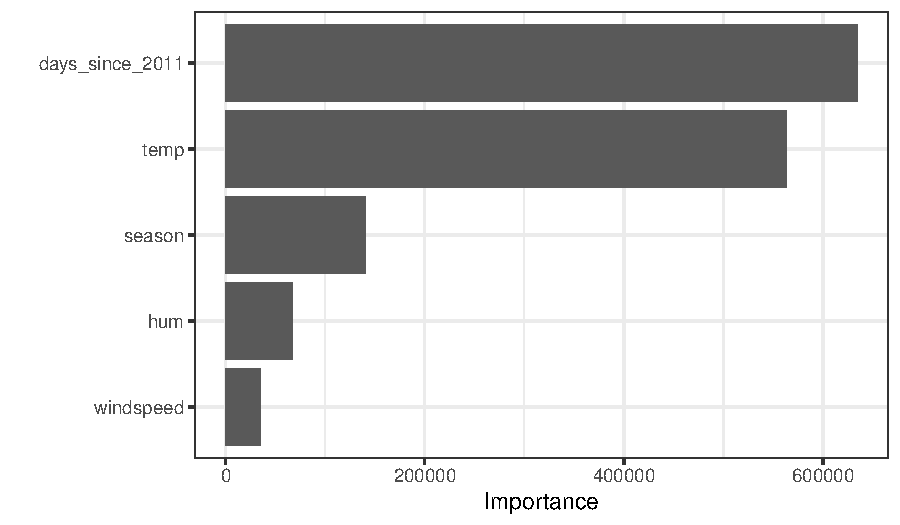
\includegraphics[width = \linewidth]{figure/compboost_pfi_base2.pdf}\\
\centering \scriptsize
In-bag-risk: 434,686.0 \\
OOB risk (10-fold CV): 446,450.0
\end{column}


\begin{column}{0.47\linewidth}
\hspace{46pt}{\scriptsize{20 iterations}}
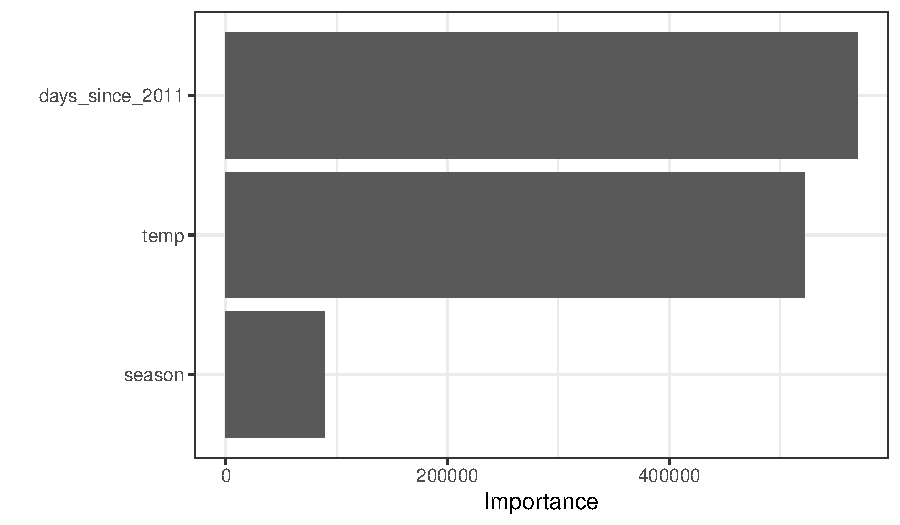
\includegraphics[width = \linewidth]{figure/compboost_pfi_base1.pdf}\\
\centering \scriptsize
In-bag-risk: 693,505.0\\
OOB risk (10-fold CV): 705,776.0
\end{column}
\end{columns}

\begin{center}
\scriptsize
$\Rightarrow$ Difference in risk: 258,819.0\\
Difference in OOB risk: 259,326.0\\
% \normalsize
% \medskip
% $\leadsto$ Ranking of features stays the same

\end{center}

\end{frame}


\begin{frame}{Non-linear Example: Interpretation}

\begin{itemize}
    \item Fit model on bike data with different BL types (1000 iter.) \citebutton{Daniel Schalk et al. 2018}{https://doi.org/10.21105/joss.00967}
    \item BLs: linear and centered splines for numeric features, categorical for season
    %and categorical base learner for season
\end{itemize}
\begin{columns}[T, totalwidth = \textwidth]
\visible<2->{
\begin{column}{0.5\linewidth}
\hspace{45pt}{\scriptsize{Feature importance}}
 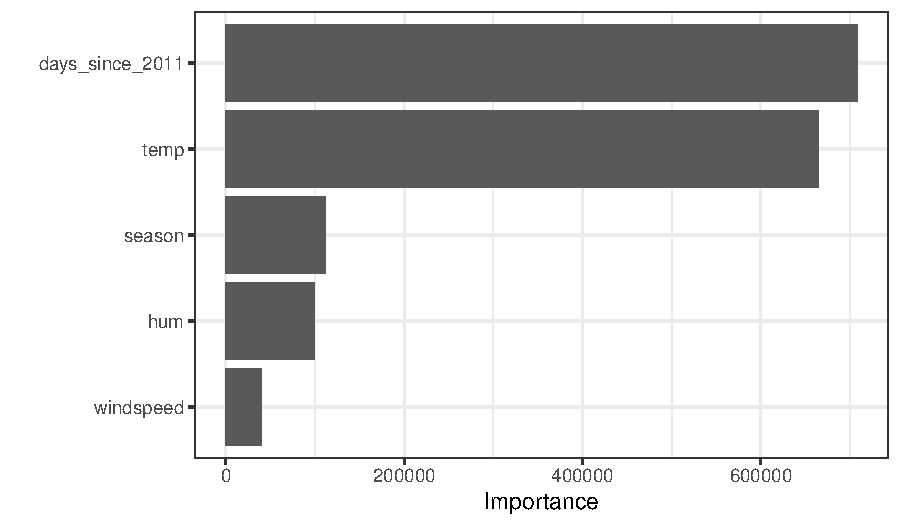
\includegraphics[width = \linewidth]{figure/compboost_pfi.pdf}
%Feature importance (risk reduction over iter.)\\
%$\leadsto$ \code{days\_since\_2011} most important
%\scriptsize
%\verbatiminput{figure/mboost_output.txt}
\end{column}
}
\visible<2->{
\begin{column}{0.5\linewidth}  %%<--- here
\hspace{23pt}{\scriptsize{Feature effect}}
  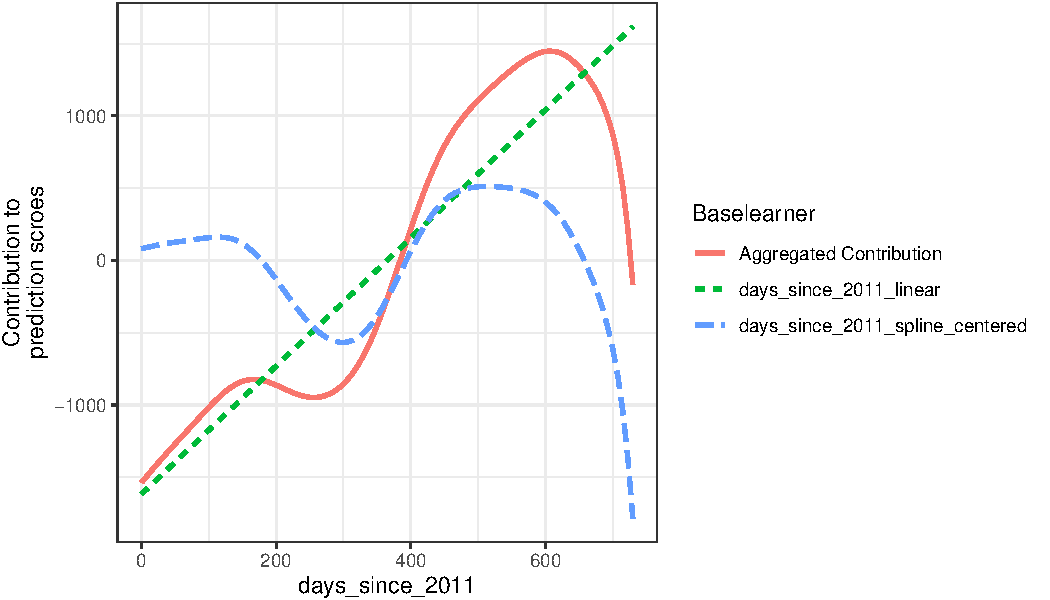
\includegraphics[width = \linewidth]{figure/compboost_pfe.pdf}
%Partial feature effect for \code{days\_since\_2011}\\
%$\leadsto$ Total effect: Combination of partial effects of linear BL and centered spline BL
\end{column}
}
\end{columns}
\smallskip
\scriptsize
\only<2->{\qquad $\Rightarrow$ In-bag-risk: 250,202.0 \, ; \, OOB risk (10-fold CV): 267,497.0 (difference to lin. example: 178,953.0)\\
\qquad $\Rightarrow$ In-bag-risk: 434,686.0 \, ; \, OOB risk (10-fold CV): 446,450.0 (previous lin. example with 1000 iter.)}
\begin{itemize}
    \normalsize
    \item<2->  Feature importance (risk reduction over iter.) \\ $\leadsto$ \code{days\_since\_2011} most important
    \item<2-> Total effect for \code{days\_since\_2011}\\
$\leadsto$ Combination of partial effects of linear BL and centered spline BL
\end{itemize}
\end{frame}

%------------------------------------------------------------------
%------------------------------------------------------------------


% \begin{frame}{Decision Trees}

% \begin{columns}[totalwidth=\textwidth]

% \begin{column}{0.3\textwidth}

%   \begin{tikzpicture}
%   \usetikzlibrary{arrows}
%     \usetikzlibrary{shapes}
%      \tikzset{treenode/.style={draw, circle, font=\small}}
%      \tikzset{line/.style={draw, thick}}
%      \node [treenode, draw=red] (a0) {$a_0$};
%      \node [treenode, below=0.75cm of a0, xshift=-1cm]  (a1) {$a_1$};
%      \node [treenode, draw=red, below=0.75cm of a0, xshift=1cm]  (a2) {$a_2$};

%      \node [treenode, draw=red, below=0.75cm of a2, xshift=-1cm] (a3) {$a_3$};
%      \node [treenode, below=0.75cm of a2, xshift=1cm]  (a4) {$a_4$};

%      \node [treenode, below=0.75cm of a3, xshift=-1cm] (a5) {$a_5$};
%      \node [treenode, below=0.75cm of a3, xshift=1cm]  (a6) {$a_6$};

%      \path [line] (a0.south) -- + (0,-0.4cm) -| (a1.north) node [midway, above] {$x_1<0.3$};
%      \path [line] (a0.south) -- +(0,-0.4cm) -|  (a2.north) node [midway, above] {$x_1\geq0.3$};

%      \path [line] (a2.south) -- + (0,-0.4cm) -| (a3.north) node [midway, above] {$x_1<0.6$};;
%      \path [line] (a2.south) -- +(0,-0.4cm) -|  (a4.north) node [midway, above] {$x_1\geq0.6$};


%      \path [line] (a3.south) -- + (0,-0.4cm) -| (a5.north) node [midway, above] {$x_2<0.2$};;
%      \path [line] (a3.south) -- +(0,-0.4cm) -|  (a6.north) node [midway, above] {$x_2\geq0.2$};

%   \end{tikzpicture}

% \end{column}

% \begin{column}{0.7\textwidth}

% Properties:
% \begin{itemize}
%     \item able to model non-linear effects
%     \item terminal nodes (aka leaf nodes) can have several observations and predicts the mean outcome over these
%     \item Applicable to regression and classification
% \end{itemize}

% Interpretation:
% \begin{itemize}
%     \item directly by following the tree (i.e., sequence of rules)
%     \item Feature importance by (scaled) score of much the splitting criterion was reduced compared to the parent
% \end{itemize}

% \end{column}

% \end{columns}

% \end{frame}

% \begin{frame}{Decision Trees \citebutton{Breiman et al. (1984)}{https://doi.org/10.1201/9781315139470}}

% %\textbf{Problem}: Can we model non-linear effects and interactions automatically (without manual specification as in GLMs or GAMs)?\\
% %Relationship between features and target are non-linear or interactions are present\\
% %\medskip
% %\pause

% \begin{columns}[T, totalwidth=\textwidth]

% \begin{column}{0.7\textwidth}
% \textbf{Idea of decision trees}: 
% %Split data in different subsets based on cut-off values in features 
% Partition data into subsets based on cut-off values in features (found by minimizing a split criterion via greedy search) and predict constant mean $c_m$ in leaf node $\mathcal{R}_m$:

% $$
% \hat f(x) = \sum_{m=1}^M c_m \mathds{1}_{\{x \in \mathcal{R}_m\}}
% $$

% % \begin{itemize}
% % \item where $c_m$ is a constant and 
% % \item $\mathcal{R}_m$ the $m$-th leaf node of the tree
% % \end{itemize}
% \pause
% \begin{itemize}
%     %\item Finding best split point (CART): Greedy search for the point that minimizes the variance of $y$ (regression) or the Gini index (classification)
%     \item Applicable to regression and classification
%     \item Able to model interactions and non-linear effects
%     \item Able to handle mixed feature spaces and missing values
% \end{itemize}

% \end{column}
% \begin{column}{0.3\textwidth}

% \begin{tikzpicture}[scale=0.75, transform shape]
%    \usetikzlibrary{arrows}
%     \usetikzlibrary{shapes}
%      \tikzset{treenode/.style={draw, circle, font=\small}}
%      \tikzset{line/.style={draw, thick}}
%      \node [treenode, draw=red] (a0) {};
%      \node [treenode, below=0.75cm of a0, xshift=-1.5cm]  (a1) {};
%      \node [treenode, below=0.75cm of a0, xshift=1.5cm]  (a2) {};

%      \node [treenode, below=0.75cm of a2, xshift=-0.75cm] (a3) {$c_1$};
%      \node [treenode, below=0.75cm of a2, xshift=0.75cm]  (a4) {$c_2$};

%     \node [treenode, below=0.75cm of a1, xshift=-0.75cm] (a5) {$c_3$};
%     \node [treenode, below=0.75cm of a1, xshift=0.75cm]  (a6) {$c_4$};

%      \path [line] (a0.south) -- + (0,-0.4cm) -| (a1.north) node [midway, above] {$x_1<3$};
%      \path [line] (a0.south) -- +(0,-0.4cm) -|  (a2.north) node [midway, above] {$x_1\geq3$};

%      \path [line] (a2.south) -- + (0,-0.4cm) -| (a3.north) node [midway, above] {$x_2<6$};;
%      \path [line] (a2.south) -- +(0,-0.4cm) -|  (a4.north) node [midway, above] {$x_2\geq6$};

%     \path [line] (a1.south) -- + (0,-0.4cm) -| (a5.north) node [midway, above] {$x_3<2$};;
%     \path [line] (a1.south) -- +(0,-0.4cm) -|  (a6.north) node [midway, above] {$x_3\geq2$};

%     %\path (a5.south) -- +(0,0) -|  (a5.south) node [midway, below] {$f_{1,3}(x_1,x_3)$};
%     %\path (a6.south) -- +(0,0) -|  (a6.south) node [midway, below] {$f_{1,3}(x_1,x_3)$};

%     %\path (a3.south) -- +(0,0) -|  (a3.south) node [midway, below] {$f_{1,2}(x_1,x_2)$};
%     %\path (a3.south) -- +(0,0) -|  (a4.south) node [midway, below] {$f_{1,2}(x_1,x_2)$};
%     % \path (a3) edge [bend right, draw=white] node [below] {$f_{1,2}(x_1,x_2)$} (a4);
%     % \path (a5) edge [bend right, draw=white] node [below] {$f_{1,3}(x_1,x_3)$} (a6);
%    \end{tikzpicture}
   
% \end{column}
% \end{columns}

% \medskip
% \pause
% \textbf{Interpretation}
% \begin{itemize}
%     \item Directly by following the tree structure (i.e., sequence of decision rules)
%     \item Importance of $x_j$: Aggregate ``improvement in split criterion'' over all splits where $x_j$ was involved\\
%     (e.g., variance for regression or Gini index for classification)
%     %Feature importance: How much did split criterion improve compared to parent node% by (scaled) score of how much splitting criterion (e.g. variance) is reduced compared to a parent node
% \end{itemize}



% \end{frame}

% \begin{frame}{Decision Trees - Example}
% \begin{itemize}
%     \item Fit decision tree with tree depth of 3 on bike data
%     \item E.g., mean prediction for the first 105 days since 2011 is 1798 (applies to $\hat = 15\%$ of the data)
%     \item \code{days\_since\_2011} shows highest feature importance (explains most of variance)
% \end{itemize}
% \begin{columns}[T, totalwidth=\textwidth]
% \begin{column}{0.4\textwidth}
% \vspace{1.5cm}
% \begin{table}[ht]
% \centering
% \begin{tabular}{lr}
%   \hline
%  Feature & Importance \\
%   \hline
% days\_since\_2011 & 79.53 \\ 
%   temp & 17.55 \\ 
%   hum & 2.92 \\ 
%    \hline
% \end{tabular}
% \end{table}
% \end{column}
% \begin{column}{0.6\textwidth}
%   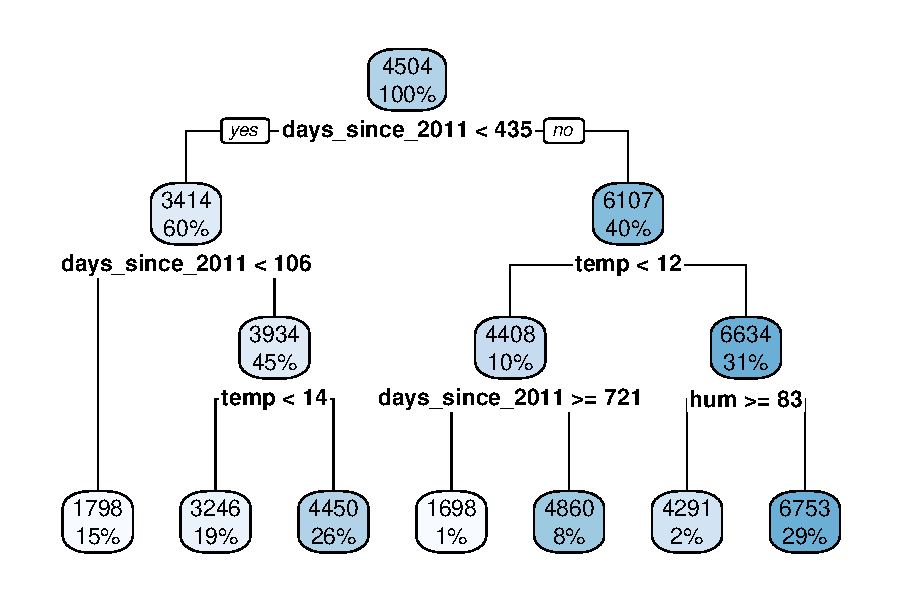
\includegraphics[width = \textwidth]{figure/tree.pdf} 
% \end{column}
% \end{columns}
 
% \end{frame}
% %------------------------------------------------------------------
% %------------------------------------------------------------------

% %\begin{frame}[c]{Decision Rules}

% %\texttt{IF COND$_1$ AND COND$_2$ AND ... THEN value}

% %\begin{itemize}
% %    \item \texttt{COND$_i$} can be of the form \texttt{feature <op> value} where \texttt{<op>} can be for example $\{=, <, > \}$
% %\end{itemize}

% %\pause
% %\medskip

% %Properties:
% %\begin{description}
% %    \item{Support} Fraction of observations to support appliance of rule
% %    \item{Accuracy} for predicting the correct class under the condition(s)
% %\end{description}

% %$\leadsto$ often trade-off between these two

% %\pause
% %\medskip

% %$\leadsto$ many different ways to learn a set of rules (incl. a default rule if none of the rules are met)

% %\end{frame}

% %------------------------------------------------------------------
% %------------------------------------------------------------------


% \begin{frame}{Other Interpretable Models}

% \begin{columns}[totalwidth=\textwidth]
%     \begin{column}{0.7\textwidth}
%         \textbf{RuleFit} \citebutton{Friedman and Popescu 2008}{https://arxiv.org/abs/0811.1679}
%         \begin{itemize}
%             \item Combination of linear models and decision trees 
%             \item Allows for feature interactions and non-linearities
%         \end{itemize}

%         \only<2->{\textbf{Decision Rules} \citebutton{Holte 1993}{https://doi.org/10.1023/A:1022631118932}
%         \begin{itemize}
%             \item Simple ``if -- then'' statements - very intuitive and easy-to-interpret
%             \item Most methods work only for classification and categorical feat.
%         \end{itemize}}

%         \only<3->{\textbf{Naive Bayes}
%         \citebutton{Zhang 2004}{https://www.aaai.org/Papers/FLAIRS/2004/Flairs04-097.pdf}
%         %$$P (C_k \mid x ) = \frac{1}{Z} P(C_k) \prod_{i=1}^{n} P(x_i \mid C_k) $$
%         \begin{itemize}
%             \item Uses Bayes' theorem to assign class prob. to observations
%             %Product of (conditional) probabilities for a class on the value of each feature
%             %For each feature, it calculates the probability for a class depending on the value of the feature. 
%             \item Strong assumption: Independence of features
%         \end{itemize}}

%         \only<4->{\textbf{k-Nearest Neighbor}
%         \citebutton{Cover 1967}{https://doi.org/10.1109/TIT.1967.1053964}
%         \begin{itemize}
%             \item (Closely related to case-based reasoning)
%             \item Average of the outcome of neighbors -- local explanation
%         \end{itemize}

%         ...}
%     \end{column}
%     \begin{column}{0.3\textwidth}
%     \vspace{\dimexpr-2\parsep-2\parskip\relax}
%         \begin{center}
%             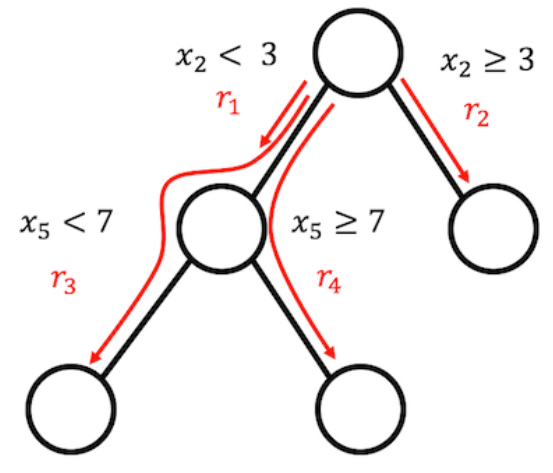
\includegraphics[width = 0.6\textwidth]{figure/RuleFit.png} \\
%             \smallskip
%             \only<2->{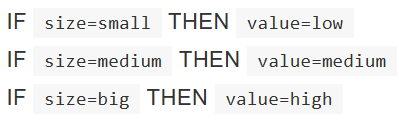
\includegraphics[width = 0.8\textwidth]{figure/decision_rules.png} \\
%             \citebutton{Molnar 2022}{https://christophm.github.io/interpretable-ml-book/}\\
%             \smallskip}
%             \only<4->{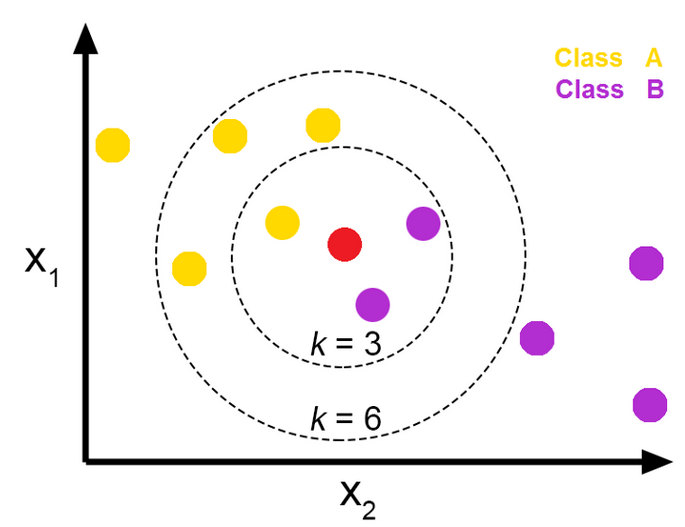
\includegraphics[width = 0.7\textwidth]{figure/knn.png} 
%             \citebutton{José 2018}{https://towardsdatascience.com/knn-k-nearest-neighbors-1-a4707b24bd1d}}
%         \end{center}
%     \end{column}
% \end{columns}

% \end{frame}


\endlecture
\end{document}
